\documentclass[twoside]{book}

% Packages required by doxygen
\usepackage{fixltx2e}
\usepackage{calc}
\usepackage{doxygen}
\usepackage[export]{adjustbox} % also loads graphicx
\usepackage{graphicx}
\usepackage[utf8]{inputenc}
\usepackage{makeidx}
\usepackage{multicol}
\usepackage{multirow}
\PassOptionsToPackage{warn}{textcomp}
\usepackage{textcomp}
\usepackage[nointegrals]{wasysym}
\usepackage[table]{xcolor}

% Font selection
\usepackage[T1]{fontenc}
\usepackage[scaled=.90]{helvet}
\usepackage{courier}
\usepackage{amssymb}
\usepackage{sectsty}
\renewcommand{\familydefault}{\sfdefault}
\allsectionsfont{%
  \fontseries{bc}\selectfont%
  \color{darkgray}%
}
\renewcommand{\DoxyLabelFont}{%
  \fontseries{bc}\selectfont%
  \color{darkgray}%
}
\newcommand{\+}{\discretionary{\mbox{\scriptsize$\hookleftarrow$}}{}{}}

% Page & text layout
\usepackage{geometry}
\geometry{%
  a4paper,%
  top=2.5cm,%
  bottom=2.5cm,%
  left=2.5cm,%
  right=2.5cm%
}
\tolerance=750
\hfuzz=15pt
\hbadness=750
\setlength{\emergencystretch}{15pt}
\setlength{\parindent}{0cm}
\setlength{\parskip}{3ex plus 2ex minus 2ex}
\makeatletter
\renewcommand{\paragraph}{%
  \@startsection{paragraph}{4}{0ex}{-1.0ex}{1.0ex}{%
    \normalfont\normalsize\bfseries\SS@parafont%
  }%
}
\renewcommand{\subparagraph}{%
  \@startsection{subparagraph}{5}{0ex}{-1.0ex}{1.0ex}{%
    \normalfont\normalsize\bfseries\SS@subparafont%
  }%
}
\makeatother

% Headers & footers
\usepackage{fancyhdr}
\pagestyle{fancyplain}
\fancyhead[LE]{\fancyplain{}{\bfseries\thepage}}
\fancyhead[CE]{\fancyplain{}{}}
\fancyhead[RE]{\fancyplain{}{\bfseries\leftmark}}
\fancyhead[LO]{\fancyplain{}{\bfseries\rightmark}}
\fancyhead[CO]{\fancyplain{}{}}
\fancyhead[RO]{\fancyplain{}{\bfseries\thepage}}
\fancyfoot[LE]{\fancyplain{}{}}
\fancyfoot[CE]{\fancyplain{}{}}
\fancyfoot[RE]{\fancyplain{}{\bfseries\scriptsize Generated by Doxygen }}
\fancyfoot[LO]{\fancyplain{}{\bfseries\scriptsize Generated by Doxygen }}
\fancyfoot[CO]{\fancyplain{}{}}
\fancyfoot[RO]{\fancyplain{}{}}
\renewcommand{\footrulewidth}{0.4pt}
\renewcommand{\chaptermark}[1]{%
  \markboth{#1}{}%
}
\renewcommand{\sectionmark}[1]{%
  \markright{\thesection\ #1}%
}

% Indices & bibliography
\usepackage{natbib}
\usepackage[titles]{tocloft}
\setcounter{tocdepth}{3}
\setcounter{secnumdepth}{5}
\makeindex

% Hyperlinks (required, but should be loaded last)
\usepackage{ifpdf}
\ifpdf
  \usepackage[pdftex,pagebackref=true]{hyperref}
\else
  \usepackage[ps2pdf,pagebackref=true]{hyperref}
\fi
\hypersetup{%
  colorlinks=true,%
  linkcolor=blue,%
  citecolor=blue,%
  unicode%
}

% Custom commands
\newcommand{\clearemptydoublepage}{%
  \newpage{\pagestyle{empty}\cleardoublepage}%
}

\usepackage{caption}
\captionsetup{labelsep=space,justification=centering,font={bf},singlelinecheck=off,skip=4pt,position=top}

%===== C O N T E N T S =====

\begin{document}

% Titlepage & ToC
\hypersetup{pageanchor=false,
             bookmarksnumbered=true,
             pdfencoding=unicode
            }
\pagenumbering{alph}
\begin{titlepage}
\vspace*{7cm}
\begin{center}%
{\Large P2P \\[1ex]\large 1 }\\
\vspace*{1cm}
{\large Generated by Doxygen 1.8.13}\\
\end{center}
\end{titlepage}
\clearemptydoublepage
\pagenumbering{roman}
\tableofcontents
\clearemptydoublepage
\pagenumbering{arabic}
\hypersetup{pageanchor=true}

%--- Begin generated contents ---
\chapter{Class Index}
\section{Class List}
Here are the classes, structs, unions and interfaces with brief descriptions\+:\begin{DoxyCompactList}
\item\contentsline{section}{\hyperlink{classclient_1_1Client}{client.\+Client} }{\pageref{classclient_1_1Client}}{}
\item\contentsline{section}{\hyperlink{classcommon_1_1Messages}{common.\+Messages} }{\pageref{classcommon_1_1Messages}}{}
\item\contentsline{section}{\hyperlink{classserveur_1_1Serveur}{serveur.\+Serveur} }{\pageref{classserveur_1_1Serveur}}{}
\item\contentsline{section}{\hyperlink{classcommon_1_1Socket}{common.\+Socket} \\*Cette classe permet de gérer les sockets }{\pageref{classcommon_1_1Socket}}{}
\end{DoxyCompactList}

\chapter{Class Documentation}
\hypertarget{classcommon_1_1GestionnaireClient}{}\section{common.\+Gestionnaire\+Client Class Reference}
\label{classcommon_1_1GestionnaireClient}\index{common.\+Gestionnaire\+Client@{common.\+Gestionnaire\+Client}}
\subsection*{Public Member Functions}
\begin{DoxyCompactItemize}
\item 
\mbox{\Hypertarget{classcommon_1_1GestionnaireClient_ac4a3e1d8fcccc18b354132893e29aac6}\label{classcommon_1_1GestionnaireClient_ac4a3e1d8fcccc18b354132893e29aac6}} 
void {\bfseries traiter\+Client} (Socket soc\+Service)
\end{DoxyCompactItemize}


The documentation for this class was generated from the following file\+:\begin{DoxyCompactItemize}
\item 
/home/seb/\+Travail/\+Dev/\+P2\+P/p2p\+\_\+stri/code/src/common/Gestionnaire\+Client.\+java\end{DoxyCompactItemize}

\hypertarget{classserveur_1_1MainServeur}{}\section{serveur.\+Main\+Serveur Class Reference}
\label{classserveur_1_1MainServeur}\index{serveur.\+Main\+Serveur@{serveur.\+Main\+Serveur}}


Classe qui permet l\textquotesingle{}execution du serveur de transfert de fichiers.  


\subsection*{Static Public Member Functions}
\begin{DoxyCompactItemize}
\item 
\mbox{\Hypertarget{classserveur_1_1MainServeur_afe17c1452f1eaafbe93c797ff10bc824}\label{classserveur_1_1MainServeur_afe17c1452f1eaafbe93c797ff10bc824}} 
static void {\bfseries main} (String\mbox{[}$\,$\mbox{]} args)
\end{DoxyCompactItemize}


\subsection{Detailed Description}
Classe qui permet l\textquotesingle{}execution du serveur de transfert de fichiers. 

The documentation for this class was generated from the following file\+:\begin{DoxyCompactItemize}
\item 
Main\+Serveur.\+java\end{DoxyCompactItemize}

\hypertarget{classcommon_1_1Messages}{}\section{common.\+Messages Class Reference}
\label{classcommon_1_1Messages}\index{common.\+Messages@{common.\+Messages}}


cette classe gère les messages d\textquotesingle{}information et d\textquotesingle{}erreurs  


\subsection*{Public Member Functions}
\begin{DoxyCompactItemize}
\item 
void \hyperlink{classcommon_1_1Messages_a6069bc66b0eda8fdd5966a7c7a8a1a0a}{ecrire\+Message} (String message)
\begin{DoxyCompactList}\small\item\em écrit un message d\textquotesingle{}information. \end{DoxyCompactList}\item 
void \hyperlink{classcommon_1_1Messages_a5d8d6f3ce6024d78171f9e49de7f6136}{ecrire\+Erreur} (String message)
\begin{DoxyCompactList}\small\item\em écrit un message d\textquotesingle{}erreur. \end{DoxyCompactList}\end{DoxyCompactItemize}
\subsection*{Static Public Member Functions}
\begin{DoxyCompactItemize}
\item 
static \hyperlink{classcommon_1_1Messages}{Messages} \hyperlink{classcommon_1_1Messages_a96928a28b3f958fc717fca2c076f773c}{get\+Instance} ()
\begin{DoxyCompactList}\small\item\em singleton pour accéder à une instance unique de \hyperlink{classcommon_1_1Messages}{Messages} \end{DoxyCompactList}\end{DoxyCompactItemize}


\subsection{Detailed Description}
cette classe gère les messages d\textquotesingle{}information et d\textquotesingle{}erreurs 

\subsection{Member Function Documentation}
\mbox{\Hypertarget{classcommon_1_1Messages_a5d8d6f3ce6024d78171f9e49de7f6136}\label{classcommon_1_1Messages_a5d8d6f3ce6024d78171f9e49de7f6136}} 
\index{common\+::\+Messages@{common\+::\+Messages}!ecrire\+Erreur@{ecrire\+Erreur}}
\index{ecrire\+Erreur@{ecrire\+Erreur}!common\+::\+Messages@{common\+::\+Messages}}
\subsubsection{\texorpdfstring{ecrire\+Erreur()}{ecrireErreur()}}
{\footnotesize\ttfamily void common.\+Messages.\+ecrire\+Erreur (\begin{DoxyParamCaption}\item[{String}]{message }\end{DoxyParamCaption})\hspace{0.3cm}{\ttfamily [inline]}}



écrit un message d\textquotesingle{}erreur. 


\begin{DoxyParams}{Parameters}
{\em message} & message à écrire \\
\hline
\end{DoxyParams}
\mbox{\Hypertarget{classcommon_1_1Messages_a6069bc66b0eda8fdd5966a7c7a8a1a0a}\label{classcommon_1_1Messages_a6069bc66b0eda8fdd5966a7c7a8a1a0a}} 
\index{common\+::\+Messages@{common\+::\+Messages}!ecrire\+Message@{ecrire\+Message}}
\index{ecrire\+Message@{ecrire\+Message}!common\+::\+Messages@{common\+::\+Messages}}
\subsubsection{\texorpdfstring{ecrire\+Message()}{ecrireMessage()}}
{\footnotesize\ttfamily void common.\+Messages.\+ecrire\+Message (\begin{DoxyParamCaption}\item[{String}]{message }\end{DoxyParamCaption})\hspace{0.3cm}{\ttfamily [inline]}}



écrit un message d\textquotesingle{}information. 


\begin{DoxyParams}{Parameters}
{\em message} & message à écrire \\
\hline
\end{DoxyParams}
\mbox{\Hypertarget{classcommon_1_1Messages_a96928a28b3f958fc717fca2c076f773c}\label{classcommon_1_1Messages_a96928a28b3f958fc717fca2c076f773c}} 
\index{common\+::\+Messages@{common\+::\+Messages}!get\+Instance@{get\+Instance}}
\index{get\+Instance@{get\+Instance}!common\+::\+Messages@{common\+::\+Messages}}
\subsubsection{\texorpdfstring{get\+Instance()}{getInstance()}}
{\footnotesize\ttfamily static \hyperlink{classcommon_1_1Messages}{Messages} common.\+Messages.\+get\+Instance (\begin{DoxyParamCaption}{ }\end{DoxyParamCaption})\hspace{0.3cm}{\ttfamily [inline]}, {\ttfamily [static]}}



singleton pour accéder à une instance unique de \hyperlink{classcommon_1_1Messages}{Messages} 

\begin{DoxyReturn}{Returns}
retourne une instance unique de \hyperlink{classcommon_1_1Messages}{Messages} 
\end{DoxyReturn}


The documentation for this class was generated from the following file\+:\begin{DoxyCompactItemize}
\item 
Messages.\+java\end{DoxyCompactItemize}

\hypertarget{classcommon_1_1Serveur}{}\section{common.\+Serveur Class Reference}
\label{classcommon_1_1Serveur}\index{common.\+Serveur@{common.\+Serveur}}


Cette classe gère les fonctionnalitées de serveur.  




Inheritance diagram for common.\+Serveur\+:
\nopagebreak
\begin{figure}[H]
\begin{center}
\leavevmode
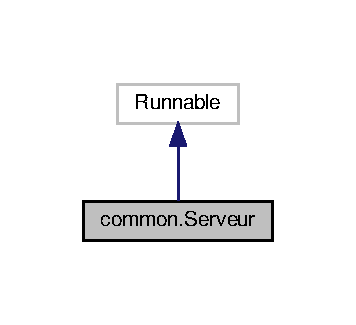
\includegraphics[width=171pt]{classcommon_1_1Serveur__inherit__graph}
\end{center}
\end{figure}


Collaboration diagram for common.\+Serveur\+:
\nopagebreak
\begin{figure}[H]
\begin{center}
\leavevmode
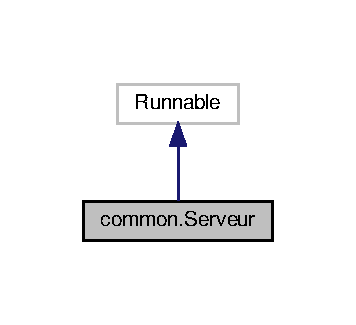
\includegraphics[width=171pt]{classcommon_1_1Serveur__coll__graph}
\end{center}
\end{figure}
\subsection*{Public Member Functions}
\begin{DoxyCompactItemize}
\item 
\hyperlink{classcommon_1_1Serveur_aef95775f670ec2ecd40e72111b125889}{Serveur} (int port, String adresse\+Dossier\+Partage)
\begin{DoxyCompactList}\small\item\em constructeur de la classe. \end{DoxyCompactList}\item 
void \hyperlink{classcommon_1_1Serveur_a14bedaf947acad1ebd395abf548b2a98}{run} ()
\begin{DoxyCompactList}\small\item\em Cette méthode permet de lancer le serveur. \end{DoxyCompactList}\end{DoxyCompactItemize}


\subsection{Detailed Description}
Cette classe gère les fonctionnalitées de serveur. 

\subsection{Constructor \& Destructor Documentation}
\mbox{\Hypertarget{classcommon_1_1Serveur_aef95775f670ec2ecd40e72111b125889}\label{classcommon_1_1Serveur_aef95775f670ec2ecd40e72111b125889}} 
\index{common\+::\+Serveur@{common\+::\+Serveur}!Serveur@{Serveur}}
\index{Serveur@{Serveur}!common\+::\+Serveur@{common\+::\+Serveur}}
\subsubsection{\texorpdfstring{Serveur()}{Serveur()}}
{\footnotesize\ttfamily common.\+Serveur.\+Serveur (\begin{DoxyParamCaption}\item[{int}]{port,  }\item[{String}]{adresse\+Dossier\+Partage }\end{DoxyParamCaption})\hspace{0.3cm}{\ttfamily [inline]}}



constructeur de la classe. 


\begin{DoxyParams}{Parameters}
{\em port} & port d\textquotesingle{}écoute du serveur. \\
\hline
{\em adresse\+Dossier\+Partage} & adresse du dossier qui contient les fichier partagés par le serveur. \\
\hline
\end{DoxyParams}


\subsection{Member Function Documentation}
\mbox{\Hypertarget{classcommon_1_1Serveur_a14bedaf947acad1ebd395abf548b2a98}\label{classcommon_1_1Serveur_a14bedaf947acad1ebd395abf548b2a98}} 
\index{common\+::\+Serveur@{common\+::\+Serveur}!run@{run}}
\index{run@{run}!common\+::\+Serveur@{common\+::\+Serveur}}
\subsubsection{\texorpdfstring{run()}{run()}}
{\footnotesize\ttfamily void common.\+Serveur.\+run (\begin{DoxyParamCaption}{ }\end{DoxyParamCaption})\hspace{0.3cm}{\ttfamily [inline]}}



Cette méthode permet de lancer le serveur. 

cette méthode lance le serveur en ouvrant la socket de rendez-\/vous, la méthode va par la suite attendre la venue d\textquotesingle{}un client puis transferer chaque connexion au gestionnaire de client pour qu\textquotesingle{}il traite les requête de chaque client dans un Thread unique. 

The documentation for this class was generated from the following file\+:\begin{DoxyCompactItemize}
\item 
Serveur.\+java\end{DoxyCompactItemize}

%--- End generated contents ---

% Index
\backmatter
\newpage
\phantomsection
\clearemptydoublepage
\addcontentsline{toc}{chapter}{Index}
\printindex

\end{document}
